\documentclass[12pt, a4paper]{article}
\usepackage[utf8x]{inputenc}
\usepackage[spanish]{babel}

\usepackage{pdfpages}

\usepackage[T1]{fontenc} %Me deja combinar la negrita con las Mayusculas

\usepackage{amsmath}
\usepackage{amsfonts}
\usepackage{amssymb}
\usepackage{bbm} %para el 1
\usepackage{mathrsfs}
% \setmathfont[version=setB,StylisticSet=1]{XITS Math}

\usepackage{graphicx} %para la imagen
\usepackage{subcaption} %para poner varias imagenes juntas
\usepackage{float}

\title{Tarea de Aprendizaje Estadístico, Teoría y aplicación}
\author{}
\date{}

\begin{document}
\begin{titlepage} %Inicio de la caratula del tp
	\centering
	  
\includegraphics[width=0.15\textwidth]{FIUBA_logo}\par
	  {\scshape\Large Universidad de Buenos Aires
      \\ Facultad de Ingenieria \par}
      {\scshape\small Año 2018 - 2er Cuatrimestre \par}
	  \vspace{1cm}
	  {\scshape\bfseries\LARGE Aprendizaje Estadístico, Teoría y aplicación\par}
	  \vspace{0.5cm}
	  \vspace{1cm}
      {\scshape\large TAREA \par}
      \vspace{0.5cm
      \raggedright}
      {\scshape\large  ALUMNOS: \par}
      \vspace{0.5cm}
    \centering
      {\normalsize  Cabrera, Mauricio Luca - Ingenieria Electrónica \#101334 \par}
      {\small  mlcabrera@fi.uba.ar \par}
	  \vspace{0.15cm}
	  {\normalsize Flores Rodríguez, José Julián - Maestría en Ingeniería Matemática \par}
      {\small  julian12310@gmail.com \par}
	  \vspace{0.15cm}
	  {\normalsize Cajachuán, Kevin - Ingeniería Informática \#98725 \par}
      {\small  kevincajachuan@hotmail.com \par}
	  \vspace{0.15cm}
	  {\normalsize Sbruzzi, José Ignacio - Ingeniería Informática \#97452 \par}
      {\small  jose.sbru@gmail.com \par}
\end{titlepage} %Cerrado de la caratula del tp
\newpage
\tableofcontents
\newpage
\section{Clase 1}

\subsection{Ejercicio 1}

Sea una función convexa $f(x)$ no negativa, $x_0$,$x_1$,$x_2$ tales que :
 		$$x_1 \leq x_0 \leq x_2$$
		$$x_0 = p_1 x_1 + p_2 x$$
		$$p_1 \geq 0, p_2 \geq 0, p_1+p_2 = 1 $$
Y sea una recta $g(x)$ tal que:
		$$g(x_0) = f(x_0)$$
		$$g(x_1) = f(x_1)$$
Probar la siguiente desigualdad:
		$$f(x_0) \leq p_1f(x_1) + p_2f(x_2)$$

La solucion de este problema es simplemente plantear $g(x) = ax+b$ y que como la función es  $f(x)$ es convexa en el intervalo $[x_1, x_1]$ vale lo siguiente.

$g(x_1) = ax_1+b = f(x_1) $ y $g(x_2) = ax_2+b = f(x_2) $ entonces $g(x_0) = g(p_1x_1+p_2x_2)=a(p_1x_1+p_2x_2)+b = ap_1x_1+ap_2x_2+b$ y como $p_1+P_2=1$ puedo multiplicar al termino $b$ por $(p_1+P_2)$ sin alterar el resultado.

Esto resulta en que $p_1x_1+ap_2x_2+b(p_1+P_2)$ con lo que queda que
	$$g(x_0) = p_1(ax_1+b)+p_2(ax_2+b) = p_1f(x_1)+p_2f(x_2)$$

Ahora como $f(x) \leq g(x) \forall x \in [x_1,x_2]$, vale la desigualdad:
	$$f(p_1 x_1 + p_2) \leq p_1f(x_1)+p_2f(x_2)$$

\subsection{Ejercicio 2 (opcional)}

Utilizando $E[f(x)m(x)] = E[Yf(x)]$, y algún artilugio que crea conveniente, demostrar que vale la siguiente ecuacion:
		$$E[\phi(x)Y|X] = \phi(x)E[Y|X]$$

\subsection{Ejercicio 3: Simulacion de 200 puntos}
Los pares ordenados fueron simulados con las siguientes condiciones:
\begin{itemize}
    \item  $X\sim\mathcal{N}(0,1)$ una variable aleatoria truncada en el intervalo $[-1,1]$.
    \item la funcion de regresión esta dado por la siguiente forma:
$$E[Y|_{X=x}]=m(x)=
\begin{cases}
    \frac{(x+2)^2}{2}   &\text{si } -1\leq x<-0,5      \\
    \frac{x}{2} + 0,875 &\text{si } -0,5\leq x \leq 0 \\
    -5(x-0,2)^2 + 1,075 &\text{si } 0 < x < 0,5       \\
    x+0,125             &\text{si } 0,5\leq x <1
\end{cases}
$$
    \item $(Y-m(X))\sim\mathcal{N}(0,\delta^2(X))$ con $\delta(X)=0.2-0.1\cos(2\pi X)$
\end{itemize}

\begin{figure}[H]
    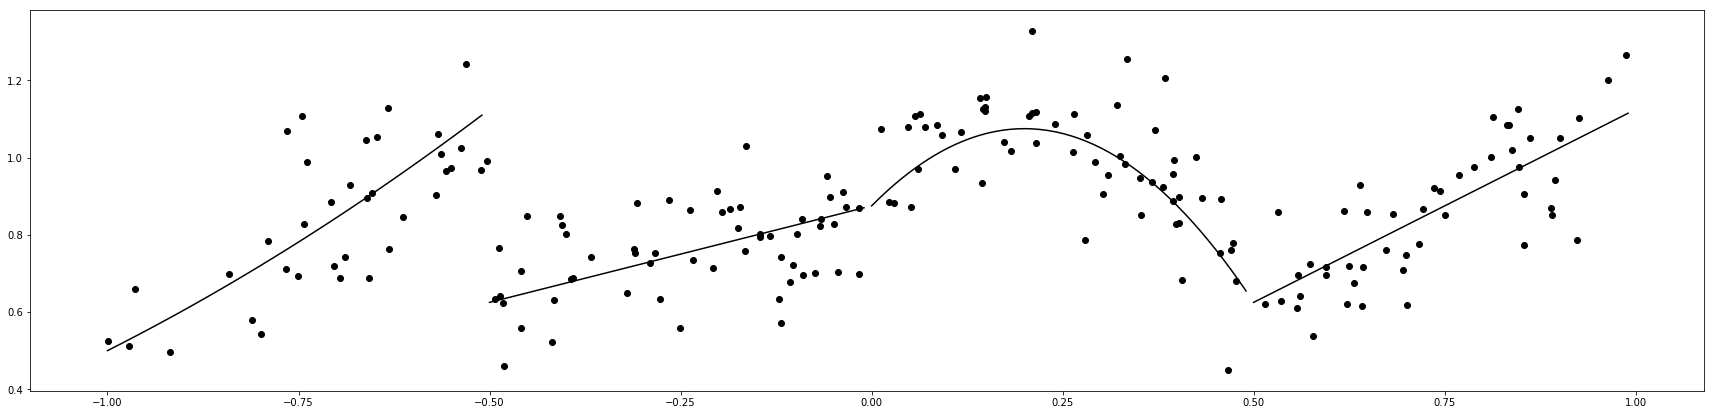
\includegraphics[width = \textwidth]{grafico}
    \caption{200 puntos simulados junto con la funcion de regresion.}
    \label{}
\end{figure}
% \includepdf[pages=-, pagecommand={}]{dato}
\subsection{Ejercicio 4: no entregable}
Dado el problema de decisión introducido en el "Diseño del receptor de una comunicación binaria", verificar que:
		$$\delta(r) = \mathbbm{1} \{ P(S=1|R=r) > P(S=0|R=r)\}$$
\section{Clase 2}
\subsection{Ejercicio 5}
Resolver la siguiente cuenta:
		$$P(X,Y) = \int\limits_0^{1/2}(1-x)\ dx + \int\limits_{1/2}^{3/4} x\ dx$$
		$$= \left.\left(x-\frac{x^2}{2}\right)\right|_{0}^{1/2}+\left. \frac{x^2}{2}\right|_{1/2}^{3/4}$$
		$$= \left(\frac{1}{2}-\frac{(1/2)^2}{2}\right) + \left(\frac{(3/4)^2}{2} - \frac{(1/2)^2}{2}\right)$$
Por lo tanto:
		$$P(X,Y) = \frac{17}{32}$$

\section{Clase 3}
\subsection{Ejercicio 8: Simulacion de Seleccion}

Abajo se simulara distantas cantidades de puntos de color y los cuales se clasificaran con distintos colores de la siguiente forma:
\begin{itemize}
	\item Se dibujan N puntos de colores, con la probabilidad de 1/2 de que sea azul y 1/2 de que sea rojo.
	\item Los rojos tendran una distribucion uniforme cubriendo un triangulo isosceles de base la recta $(0,0)\rightarrow(1,0)$ y de altura $1$
	\item Los azules tendran una distribucion uniforme cubriendo un triangulo isosceles de base la recta $(0,1)\rightarrow(1,1)$ y de altura $-1$
	\item Al terminar de pintar los puntos, usando la regla del histograma, se crearan una cuadrilla que posteriorente se pintaran de un color dependiendo de cuantos colores entraron ahi.
\end{itemize}

Para esta simulacion uso $h_n = \frac{1}{\sqrt[3]{n}}$ y se uso el siguiente criterio para la clasicacion:
		$$g_n(X)=
		\begin{cases}
		    1   &\text{si } \sum\limits_{i = 0}^{n}\mathbbm{1}\{Y=1\}\mathbbm{1}\{X_i \in A(x)\} \geq \sum\limits_{i = 0}^{n}\mathbbm{1}\{Y=0\}\mathbbm{1}\{X_i \in A(x)\}      \\
		    0 &\text{e.o.c}
		\end{cases}
		$$
\begin{center}
	\begin{figure}[H]
	    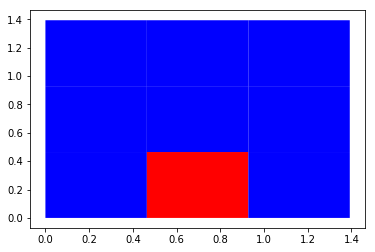
\includegraphics[width = 0.8\textwidth]{grafico_10_puntos}
	    \caption{Imagen del espacio clasificado con 10 puntos.}
	\end{figure}

	\begin{figure}[H]
	    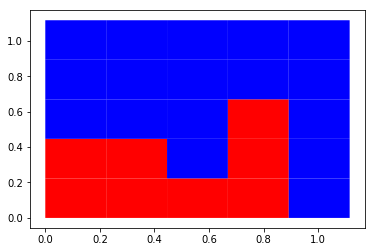
\includegraphics[width = 0.8\textwidth]{grafico_100_puntos}
	    \caption{Imagen del espacio clasificado con 100 puntos.}
	\end{figure}

	\begin{figure}[H]
	    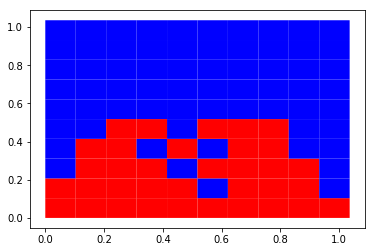
\includegraphics[width = 0.8\textwidth]{grafico_1000_puntos}
	    \caption{Imagen del espacio clasificado con 1000 puntos.}
	\end{figure}

	\begin{figure}[H]
	    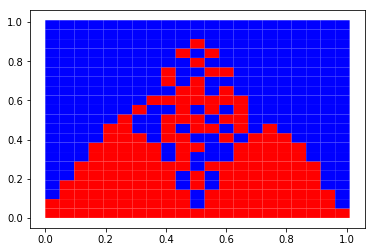
\includegraphics[width = 0.8\textwidth]{grafico_10000_puntos}
	    \caption{Imagen del espacio clasificado con 10000 puntos.}
	\end{figure}

	\begin{figure}[H]
	    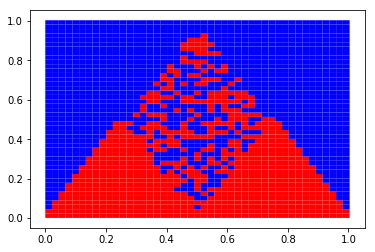
\includegraphics[width = \textwidth]{grafico_100000_puntos}
	    \caption{Imagen del espacio clasificado con 100000 puntos.}
	\end{figure}
\end{center}


\section{Clase 4}
\subsection{Ejercicio 9: Seleccion Método de los k-primeros Vecinos}

Abajo se simulara distantas cantidades de puntos de color y los cuales se clasificaran con distintos colores de la siguiente forma:
\begin{itemize}
	\item Se dibujan 50 puntos de color rojo y 50 puntos de puntos de color azul, seguido de N puntos aleatorios los cuales se decidira su color con en base a 100 puntos nombrados.
	\item Los rojos tendran una distribucion normal multivariada de la forma $\mathcal{N}((-1,0),
    \left(
        \begin{array}{c c}
            1 & 0 \\
            0 & 1
        \end{array}
    \right)
    )$
	\item Los azules tendran una distribucion normal multivariada de la forma $\mathcal{N}((1,0),
    \left(
        \begin{array}{c c}
            1 & 0 \\
            0 & 1
        \end{array}
    \right)
    )$
	\item Los puntos aleatorios tienen coordenadas $X,Y\sim\mathcal{U}(-4,4)$
\end{itemize}
Ahora el criterio de evaluacion va ser el de los k-primeros vecinos, en el que consiste revisando una cantidad k de vecinos, elegir de que color es el punto evaluado. El experimento se realizara con k = 1, 3 y 13. La cantidad de puntos N = 100, 1000, 10000, 100000.


\begin{figure}[H]
	\begin{minipage}[b]{.3\linewidth}
		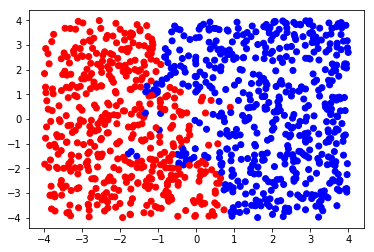
\includegraphics[width = \textwidth]{mil_puntos_1_vecino}
		\subcaption{Clasificado usando 1 vecino.}\label{fig:mil_1}
	\end{minipage}
	\begin{minipage}[b]{.3\linewidth}
		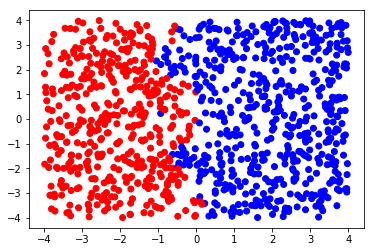
\includegraphics[width = \textwidth]{mil_puntos_3_vecino}
		\subcaption{Clasificado usando 3 vecinos.}\label{fig:mil_3}
	\end{minipage}
	\begin{minipage}[b]{.3\linewidth}
		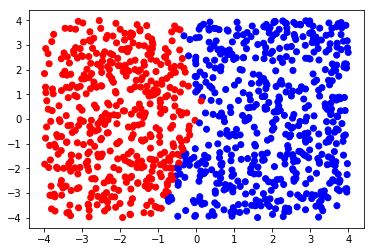
\includegraphics[width = \textwidth]{mil_puntos_13_vecino}
		\subcaption{Clasificado usando 13 vecinos.}\label{fig:mil_13}
	\end{minipage}
	\caption{Simulacion usando mil puntos}\label{fig:mil}
\end{figure}


\begin{figure}[H]
	\begin{minipage}[b]{.3\linewidth}
		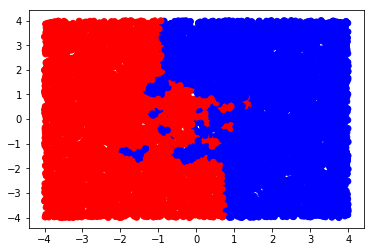
\includegraphics[width = \textwidth]{diez_mil_puntos_1_vecino}
		\subcaption{Clasificado usando 1 vecino.}\label{fig:diez_mil_1}
	\end{minipage}
	\begin{minipage}[b]{.3\linewidth}
		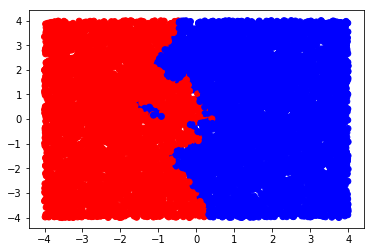
\includegraphics[width = \textwidth]{diez_mil_puntos_3_vecino}
		\subcaption{Clasificado usando 3 vecinos.}\label{fig:diez_mil_3}
	\end{minipage}
	\begin{minipage}[b]{.3\linewidth}
		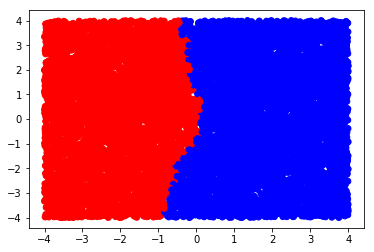
\includegraphics[width = \textwidth]{diez_mil_puntos_13_vecino}
		\subcaption{Clasificado usando 13 vecinos.}\label{fig:diez_mil_13}
	\end{minipage}
	\caption{Simulacion usando diez mil puntos}\label{fig:diez_mil}
\end{figure}

\begin{figure}[H]
	\begin{minipage}[b]{.3\linewidth}
		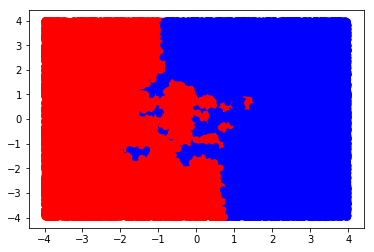
\includegraphics[width = \textwidth]{cien_mil_puntos_1_vecino}
		\subcaption{Clasificado usando 1 vecino.}\label{fig:cien_mil_1}
	\end{minipage}
	\begin{minipage}[b]{.3\linewidth}
		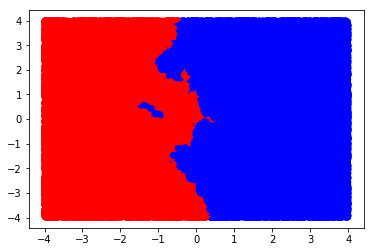
\includegraphics[width = \textwidth]{cien_mil_puntos_3_vecino}
		\subcaption{Clasificado usando 3 vecinos.}\label{fig:cien_mil_3}
	\end{minipage}
	\begin{minipage}[b]{.3\linewidth}
		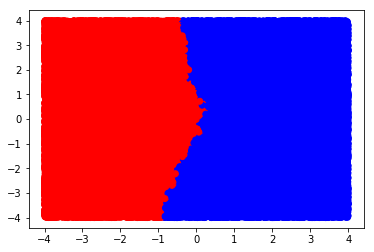
\includegraphics[width = \textwidth]{cien_mil_puntos_13_vecino}
		\subcaption{Clasificado usando 13 vecinos.}\label{fig:cien_mil_13}
	\end{minipage}
	\caption{Simulacion usando cien mil puntos}\label{fig:cien_mil}
\end{figure}

\subsection{Ejercicio 10}

Desmostrar:
		$$(a+b+c)^2 \leq 3(a^2+b^2+c^2) \forall a,b,c \in \mathbbm{R}$$
Desmostracion:

Distribuyendo el cuadrado en el trinomio resulta en lo siguiente:
		$$a^2+2ab+2ac+b^2+2bc+c^2 \leq 3(a^2+b^2+c^2)$$
		$$(a^2+b^2+c^2)+2ab+2ac+2bc \leq 3(a^2+b^2+c^2)$$
		$$2ab+2ac+2bc \leq 2(a^2+b^2+c^2)$$
Para simplificar las cuentas, reescribo a y c como $a = b+\alpha$ y $c = b+\beta$  $\forall \alpha, \beta \in \mathbbm{R}$. Quedando la entonces como:
		$$b^2+\alpha b+b^2+\beta b+\alpha b+\alpha \beta+b^2+\beta b \leq b^2+2\alpha b+\alpha^2+b^2+b^2+2\beta b+\beta^2$$
resultando en:
		$$\alpha \beta \leq \alpha^2+\beta^2$$
Lo cual es siempre verdadero $\forall \alpha,\beta \in \mathbbm{R}$.

\section{Clase 5}
\subsection{Ejercicio 11}
Dada las desigualdades:
		$$P[S_n - E[S_n] \leq \epsilon ] \geq e^{-2\epsilon/\sum\limits_{i=1}^{n}(b_i-a_i)^2}$$
		$$P[S_n - E[S_n] \geq -\epsilon ] \geq e^{-2\epsilon/\sum\limits_{i=1}^{n}(b_i-a_i)^2}$$
Probar que es obvio lo siguiente:
		$$P[|S_n - E[S_n]| > \epsilon ] \geq 2 e^{-2\epsilon/\sum\limits_{i=1}^{n}(b_i-a_i)^2}$$
Solucion, usando la propiedad $P(A\cup B) \leq P(A) + P(B)$ puedo escribir las dos ecuaciones de la siguiente forma:
		$$P[S_n - E[S_n] \leq \epsilon \cup S_n - E[S_n] \geq -\epsilon ] \leq P[S_n - E[S_n] \leq \epsilon ] + P[S_n - E[S_n] \geq -\epsilon ]$$
		$$\leq e^{-2\epsilon/\sum\limits_{i=1}^{n}(b_i-a_i)^2} + P[S_n - E[S_n] \geq -\epsilon ]$$
		$$\leq 2 e^{-2\epsilon/\sum\limits_{i=1}^{n}(b_i-a_i)^2}$$
Y que inicialmente tengo la $P[-\epsilon \leq S_n - E[S_n] \leq \epsilon ]$ lo tanto:
		$$P[|S_n - E[S_n]| > \epsilon ] \geq 2 e^{-2\epsilon/\sum\limits_{i=1}^{n}(b_i-a_i)^2}$$

\subsection{Ejercicio 12}
Probar la siguiente desigualdad:
		$$|\widehat{L}_n(\phi_n^*)-L(\phi_n^*)| \leq \sup\limits_{\phi \in \mathscr{C}}|\widehat{L}_n(\phi)-L(\phi)| $$
Basicamente dice que la que la diferencia entre el minimo error estimado, y el verdadero (basado en los datos), es menor  o igual la maxima diferencia que puede haber entre el error estimado y el verdadero para un clasificador determinado.
\subsection{Ejercicio 14: Simulacion de error}

\section{Clase 6}
\subsection{Ejercicio 16}
Para un conjunto $A' = \{(a,b): a<b \}$, calcular $N_{A'}(z_1,z_2,z_3)$

Los conjuntos que se pueden hacer son $\{\emptyset\}$, $\{z_1\}$, $\{z_2\}$, $\{z_3\}$, $\{z_1,z_2\}$, $\{z_2,z_3\}$, $\{z_1, z_2, z_3\}$. Por lo tanto $N_{A'}(z_1,z_2,z_3) = 7$

\end{document}
